\documentclass{article}\usepackage[]{graphicx}\usepackage[]{color}
%% maxwidth is the original width if it is less than linewidth
%% otherwise use linewidth (to make sure the graphics do not exceed the margin)
\makeatletter
\def\maxwidth{ %
  \ifdim\Gin@nat@width>\linewidth
    \linewidth
  \else
    \Gin@nat@width
  \fi
}
\makeatother

\definecolor{fgcolor}{rgb}{0.345, 0.345, 0.345}
\newcommand{\hlnum}[1]{\textcolor[rgb]{0.686,0.059,0.569}{#1}}%
\newcommand{\hlstr}[1]{\textcolor[rgb]{0.192,0.494,0.8}{#1}}%
\newcommand{\hlcom}[1]{\textcolor[rgb]{0.678,0.584,0.686}{\textit{#1}}}%
\newcommand{\hlopt}[1]{\textcolor[rgb]{0,0,0}{#1}}%
\newcommand{\hlstd}[1]{\textcolor[rgb]{0.345,0.345,0.345}{#1}}%
\newcommand{\hlkwa}[1]{\textcolor[rgb]{0.161,0.373,0.58}{\textbf{#1}}}%
\newcommand{\hlkwb}[1]{\textcolor[rgb]{0.69,0.353,0.396}{#1}}%
\newcommand{\hlkwc}[1]{\textcolor[rgb]{0.333,0.667,0.333}{#1}}%
\newcommand{\hlkwd}[1]{\textcolor[rgb]{0.737,0.353,0.396}{\textbf{#1}}}%
\let\hlipl\hlkwb

\usepackage{framed}
\makeatletter
\newenvironment{kframe}{%
 \def\at@end@of@kframe{}%
 \ifinner\ifhmode%
  \def\at@end@of@kframe{\end{minipage}}%
  \begin{minipage}{\columnwidth}%
 \fi\fi%
 \def\FrameCommand##1{\hskip\@totalleftmargin \hskip-\fboxsep
 \colorbox{shadecolor}{##1}\hskip-\fboxsep
     % There is no \\@totalrightmargin, so:
     \hskip-\linewidth \hskip-\@totalleftmargin \hskip\columnwidth}%
 \MakeFramed {\advance\hsize-\width
   \@totalleftmargin\z@ \linewidth\hsize
   \@setminipage}}%
 {\par\unskip\endMakeFramed%
 \at@end@of@kframe}
\makeatother

\definecolor{shadecolor}{rgb}{.97, .97, .97}
\definecolor{messagecolor}{rgb}{0, 0, 0}
\definecolor{warningcolor}{rgb}{1, 0, 1}
\definecolor{errorcolor}{rgb}{1, 0, 0}
\newenvironment{knitrout}{}{} % an empty environment to be redefined in TeX

\usepackage{alltt}
\usepackage{Sweave}
\usepackage{float}
\usepackage{graphicx}
\usepackage{tabularx}
\usepackage{siunitx}
\usepackage{geometry}
\usepackage{pdflscape}
\usepackage{mdframed}
\usepackage{natbib}
\bibliographystyle{..//refs/styles/besjournals.bst}
\usepackage[small]{caption}
\setkeys{Gin}{width=0.8\textwidth}
\setlength{\captionmargin}{30pt}
\setlength{\abovecaptionskip}{0pt}
\setlength{\belowcaptionskip}{10pt}
\topmargin -1.5cm        
\oddsidemargin -0.04cm   
\evensidemargin -0.04cm
\textwidth 16.59cm
\textheight 21.94cm 
%\pagestyle{empty} %comment if want page numbers
\parskip 7.2pt
\renewcommand{\baselinestretch}{1.5}
\parindent 0pt

\newmdenv[
  topline=true,
  bottomline=true,
  skipabove=\topsep,
  skipbelow=\topsep
]{siderules}

%% R Script


\IfFileExists{upquote.sty}{\usepackage{upquote}}{}
\begin{document}
\title{Rethinking False Spring Risk}
\author{C. J. Chamberlain $^{1,2}$, E. M. Wolkovich $^{1,2}$, B. I. Cook $^{3}$, I. Garcia de Cortazar Atauri $^{4}$}
\date{\today}
\maketitle 
 

\renewcommand{\thetable}{\arabic{table}}
\renewcommand{\thefigure}{\arabic{figure}}
\renewcommand{\labelitemi}{$-$}

%%%%%%%%%%%%%%%%%%%%%%%%%%%%%%%%%%%%%%%%%%%%%%%
\section*{Introduction}
\begin{enumerate}
\item Introduce False Spring Concept
\begin {enumerate}
\item Plants growing in temperate environments are at risk of being exposed to late spring freezes, which can be detrimental to growth. 
\item Individuals that leaf out before the last frost are at risk of leaf loss, damaging wood tissue, and slowed or stalled canopy development \citep{Gu2008, Hufkens2012}. 
\item Therefore, temperate deciduous tree species must have plastic phenological responses in the spring in order to optimize photosynthesis and minimize frost or drought risk \citep{Polgar2011}. 
\item These late spring freezing events are known as false springs. False spring events can result in highly adverse ecological and economic consequences \citep{Knudson2012, Ault2013}.
\end{enumerate}
\item Introduce Climate Change and Importance of False Spring Studies
\begin{enumerate}
\item Climate change is expected to increase damage from false spring events around the world due to earlier spring onset and greater fluctuations in temperature \citep{Cannell1986, Inouye2008, Martin2010}. 
\item Temperate forest species around the world are initiating leaf out about 4.6 days earlier per degree Celsius \citep{Wolkovich2012, Polgar2014}. 
\item It is anticipated that there will be a decrease in false spring frequency overall but the magnitude of temperature variation is likely to increase, therefore amplifying the expected intensity of false spring events \citep{Kodra2011, Allstadt2015}. 
\item Multiple studies have documented false spring events in recent years \citep{Gu2008, Augspurger2009, Knudson2012, Augspurger2013} and some have linked this to climate change \citep{Ault2013, Allstadt2015, Muffler2016, Xin2016}. 
\item Due to these reasons, it is crucial for researchers to properly evaluate the effects of false spring events on temperate forests and agricultural crops in order to make more accurate predictions on future trends.
\end{enumerate}

\item Introduce Current False Spring Index Equation
\begin{enumerate}
\item Different species respond differently to late spring freezing events. 
\item The level of damage sustained by plants from a false spring also varies across phenophases. 
\item Various studies have assessed the risk of damage or the intensity of particular false spring events but at this time false spring studies fail to incorporate all potential factors that could affect the level of frost damage risk. 
\item A False Spring Index (FSI) signifies the likelihood of a damage to occur from a late spring freeze. 
\item Currently, FSI evaluates day of budburst, number of growing degree days, and day of last spring freeze through a simple equation as seen below \citep{Marino2011}. 
\begin{equation} \label{eq:1}
FSI = Julian Date (Last Spring Freeze) - Julian Date (Budburst)
\end{equation}
\item False spring studies largely simplify the various ecological elements that could predict the level of plant damage from late spring freezing events. 
\item In contrast to these simplifications, we argue that a wealth of factors greatly impacts plants' frost spring risk such that simple indices will most likely lead to inaccurate predictions and ultimately do little to advance the field. 
\end{enumerate}

\item State the Purpose of the Paper
\begin{enumerate}
\item In this paper we aim to highlight the complexity of factors driving a plant's false spring risk. 
\item We outline in particular how life stage of the individual \citep{Caffarra2011}, location within a forest or canopy \citep{Augspurger2013}, winter chilling hours (Flynn \& Wolkovich 2017?), proximity to water \citep{Gu2008}, level of precipitation prior to the freezing event \citep{Anderegg2013}, freeze duration/intensity, and range limits of the species \citep{Martin2010} unhinge simple metrics of false spring. 
\item The ultimate intent is to demonstrate how an integrated view of false spring that incorporates these factors would rapidly advance progress in this field.  
\end{enumerate}
\end{enumerate}

%%%%%%%%%% DEFINING FALSE SPRING %%%%%%%%%%%%%
\section*{Defining False Spring}
\begin{enumerate}
\item Definition and Threat
\begin{enumerate}
\item Temperate forest plants are most at risk to frost damage from episodic spring frosts  \citep{Sakai1987}. 
\item Abnormally warm conditions in the late winter or early spring can cause budburst to initiate early in trees and shrubs.
\item Freezing temperatures following a warm spell could result in plant damage or even death \citep{Ludlum1968, Mock2007}.
\item False springs are defined by two phases: rapid vegetative growth prior to a freeze and a post freeze setback \citep{Gu2008}.
\item Freeze and thaw fluctuations can cause defoliation, xylem embolism and decreased xylem conductivity which can result in crown dieback \citep{Gu2008}.
\item Species that are better able to phenologically track the shifts in spring advancement due to climate change are more likely to sustain damaging events such as false springs \citep{Scheifinger2003}.
\end {enumerate}

\item Define Chilling requirements to specify timing of damaging false spring events
\begin {enumerate}
\item Deciduousness and the evolution of two dormancy phases (i.e. endodormancy and ecodormancy) in temperate forest trees has permitted species to occupy more northern ecological niches \citep{Samish1954}.
\item Endodormancy is the period of winter when temperate trees are inhibited from growing, regardless of the outdoor environment.
\item Ecodormancy is the period of time when growth can occur but the external environment is not conducive to growth (e.g. too cold) \citep{Basler2012}.
\item Therefore, warm temperatures earlier in the year (i.e. in February) do not seem to affect species, most likely because trees have not yet left the endodormancy phase.
\item Frost damage usually occurs when there is a warmer than average March, a freezing April, and enough growing degree days between budburst and the last freeze date \citep{Augspurger2013}.
\item A damaging false spring is currently defined as having 7 or more days between budburst and the last freeze date (Equation \ref{eq:1}) \citep{Peterson2014}.
\item The 7 day parameter exposes less resistant foliate phenophases to a false spring, thus putting the plant at a higher risk of damage. 
\item Once budburst has initiated, buds cannot respond to cold temperatures and freeze resistance is greatly reduced \citep{Taschler2004, Lenz2013, Vitasse2014}.
\item There are two types of freezes: a ``hard freeze" at -2.2$^{\circ}$C and a ``soft freeze" at -1.7$^{\circ}$C \citep{Vavrus2006, Kodra2011, Augspurger2013}.
\item However, the definition is still largely under debate. 
\end{enumerate}

\item Damage and drought
\begin{enumerate}
\item Freezing damage can occur directly via intracellular ice formation or indirectly via freezing dehydration \citep{Pearce2001, Beck2004, Hofmann2015}.
\item Intracellular ice formation often results in defoliaiton and increased xylem cavitation or embolism in the stem.
\item Freezing tolerance in plants is usually against extracellular freezing or freezing dehydration \citep{Burke1976}.
\item Drought and desiccation within the xylem mimick the adverse effects of false spring events \citep{Cavender2015}.
\item Dry winters typically result in new, frost-tolerant shoots due to the decreased water content and osmotic potential from the reduced number of accumulated solutes \citep{Morin2007, Hofmann2015}.
\item Therefore, it is hypothesized that increased bud dehydration results in increased frost hardiness \citep{Beck2007, Nielsen2009, Poirier2010, Kathke2011, Hofmann2015}, although long-term drought stress can lead to accumulated xylem damage and decreased false spring tolerance \citep{Anderegg2013}.
\item More studies are needed to investigate the interplay between false spring events and precipiation and how that relationship impacts the level and type of damage a plant sustains and what the long-term implications may be. 
\end{enumerate}
\end{enumerate}

%%%%%%%%%% DETERMINING SPRING ONSET %%%%%%%%%%%%%
\section*{Determining Spring Onset}
\begin{enumerate}
\item Elucidate the difference between spring onset and study species
\begin{enumerate}
\item Spring forest phenology essentially progresses through successional stages: understory species, seedlings and saplings typically initiate budburst first in order to exploit open canopies and early growth, whereas late successional species may start later in the season to avoid frost or drought risk \citep{Richardson2009, Xin2016}.
\item Therefore, habitat type plays a large role in the overall spring onset of a specific ecological region. 
\item Pure grasslands or young forest will, overall, have earlier budburst dates than large stands of canopy trees and mixed forests may have a spring onset date somewhere between the two.
\item False spring studies should first assess the forest demographics and functional groups of the study species in order to effectively estimate the date of spring onset.
\end{enumerate}
\item Methodologies
\begin{enumerate}
\item A suitable methodology for determining spring onset is crucial in order to establish an effective model for false spring risk, especially since the current false spring equation only uses two inputs: date of spring onset and date of last freeze (Equation \ref{eq:1}). 
\item If the date of spring onset is inaccurate, the level of risk determined by the current equation (Equation \ref{eq:1}) could render erroneous results. 
\item There are many methods available to ascertain the first day of spring.
\item Spring onset can be calculated through observational data, PhenoCam or remote-sensing data, or through the USA National Phenology Network's (USA-NPN) Extended Spring Index (SI-x) tool \citep{USA-NPN2016}.
\item Studies often use observation data to evaluate spring onset to target budburst more precisely, however, it can be difficult or even impossible for large-scale studies. 
\item PhenoCam and remote-sensing data is suitable for canopy tree species, whereas USA-NPN SI-x is more applicable for understory species. 
\item The three methodologies to determine spring onset were compared using observational data from Harvard Forest \citep{Okeefe2014}, PhenoCam data from Harvard Forest \citep{Richardson2015}, and USA-NPN SI-x \citep{USA-NPN2016} and then inputted into the FSI equation (Equation \ref{eq:1}) to calculate FSI values from 2008 to 2014 (Figure \ref{fig:fsifig}).


\begin{figure}[H]
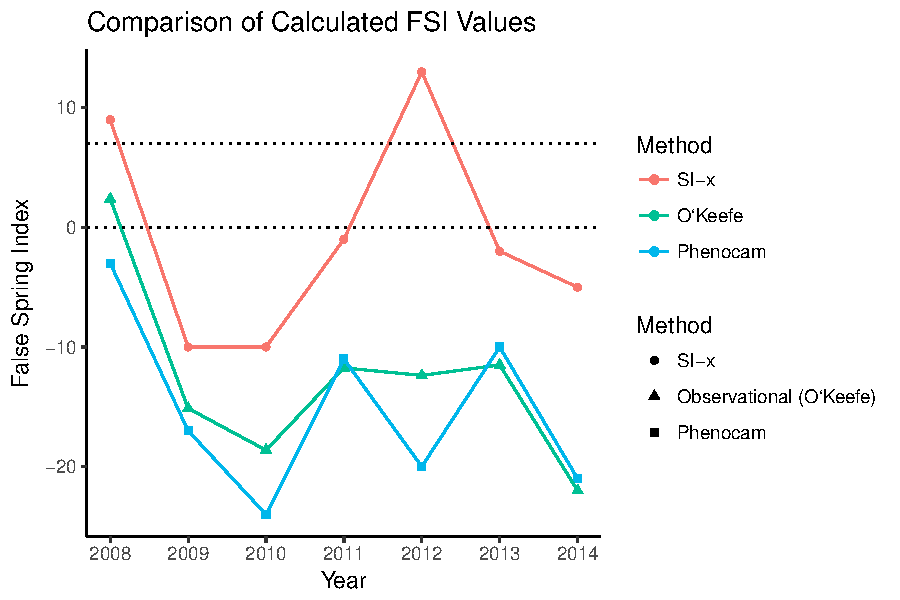
\includegraphics[width=\maxwidth]{figure/fsifig-1} \caption[A scatterplot indicating FSI values from 2008 to 2014 for each methdology used in this study]{A scatterplot indicating FSI values from 2008 to 2014 for each methdology used in this study. PhenoCam FSI values are red, Observed FSI values are blue, and USA-NPN FSI values are green.}\label{fig:fsifig}
\end{figure}



\item Observational FSI values and USA-NPN FSI values are highly comparable and are justifiable methods for determining potenial false spring risk.
\item PhenoCam data is also comparable to the other two methods, however, it would be more useful for canopy species, which is evident from the results seen in 2012 (Figure \ref{fig:fsifig}).
\item In 2012, a false spring event was reported through many regions of the US due to warm temperatures occuring in March \citep{Ault2015}.
\item These high temperatures would most likely be too early for larger canopy species to initiate budburst but they would affect smaller understory species as is seen by the discrepany in results for 2012 (Figure \ref{fig:fsifig}).
\item Researchers should use the USA-NPN dataset for understory species, PhenoCam or remote-sensing data for late successional species, and observational data for a wide array of plant functional types.
\end{enumerate}
\end{enumerate}

%%%%%%%%%% Understanding (Defining?) Vegetative Risk %%%%%%%%%%%%%
\section*{Defining Vegetative Risk}
\begin{enumerate}
\item Define Vegetative Risk
\begin {enumerate}
\item Plants at certain vegetative phenophases (i.e. before full leafout of the entire plant) are more likely to sustain damage from a false spring than individuals past the leafout phenophase. 
\item Frost tolerance steadily decreases after budburst begins until the leaf is fully unfolded, with leafout being the most susceptible to frost damage \citep {Lenz2016}.
\item The rate of budburst and the length of time between budburst and leafout is essential for predicting level of damage from a false spring event.
\item We will refer to the timing of these collective phenophases (i.e. budburst to leafout) as the duration of vegetative risk.
\end {enumerate}
\item Phenophases and Life Stage
\begin {enumerate}
\item Reproductive phases are generally more sensitive to false spring events than vegetative phases and developing leaves are more susceptible to damage than opening buds or expanding shoots \citep{Augspurger2009, Lenz2013}.
\item However, trees that suffer severe vegetative growth damage will suffer greater long-term effects from the loss of photosynthetic tissue than trees that lose one year of reproductive growth. 
\item Spring freezing events that occur during the vegetative growth phenophases impose the greatest freezing threat to deciduous tree and shrub species \citep{Sakai1987}.
\item Therefore, phenophase is a crucial indicator for how much damage a plant will sustain from a freezing event.
\item Seedlings and saplings initiate budburst before canopy closure in order to benefit from the increased light levels \citep {Augspurger2008}, which puts them at greater risk to false spring damag than adult trees \citep{Vitasse2014}.
\item Younger plants are mre likely to sustain lasting damage to the leaf buds and vegetative growth, whereas adult trees are at risk of xylem embolism.
\item For xylem embolism to occur, extreme cavitation must first be present.
\item Extensive cavitation in the xylem requires more intensive freezing events than freezing events that damage seedling and sapling leaf buds.
\item Especially strong freezing events (i.e. > -8.6$^{\circ}$C), could result in meristemic tissue, wood parenchyma and phloem damage \citep{Sakai1987, Augspurger2011, Lenz2013}.
\end{enumerate}
\item Species Differences
\begin {enumerate}
\item Different species respond differently to anthropogenic climate change.
\item Most species are expected to begin leafout earlier in the season with warming spring temperatures but some species may have the opposite response \citep{Cleland2006, Yu2010, Xin2016}.
\item Studies indicate that species growing at more northern latitudes tend to respond greater to photoperiod than species growing further south \citep {Partanen2004, Viheraaarnio2006, Caffarra2011}.
\item Similarly, late successional species exhibit greater photoperiod sensitivies than pioneer or understory species \citep{Basler2012} and they also require more chilling in the winter and greater forcing temperatures in the spring to initiate budburst \citep{Laube2013}.
\item It is anticipated that these more opportunistic individuals that initiate budburst earlier in the spring with the shifts in climate would attempt to limit freezing risk by decreasing the duration of vegetative risk and progress to full leaf expansion faster.
\item The duration of vegetative risk is usually extended if a freezing event occurs during the phenophases between budburst and full leafout and species with short durations of vegetative risk often sustain higher levels of damage \citep {Augspurger2009}.
\item It is hypothesized that if the duration of vegetative risk is longer, then the buds and leaves will be heartier against frosts, however this still has yet to be tested thoroughly.
\item We assess the interaction between duration of vegetative risk and false spring events using two datasets: from a growth chamber chilling experiment and long-term observational data.
\end {enumerate}


\item Dan's Data
\begin{enumerate}
\item Deciduous trees and shrubs require a certain number of chilling units in order to leave the endodormancy phase. 
\item This helps protect temperate plants against stochastic warm spells in the winter so that they do not break dormancy too early in the season.
\item Chilling units differ across species and across habitats.
\item Species growing at higher latitudes are more likely to have lower chilling requirements to break dormancy \citep{Myking1995, Howe2003} due to the shorter growing season and selective pressure to initiate budburst as soon as temperatures are conducive to growth \citep{Prevey2017}. % Lizzie, should I avoid this Prevey reference?
\item With anthropogenic climate change, it is possible that certain species will have insufficient winter chilling (especially at lower latitudes) resulting in higher spring forcing requirements \citep{McCreary1990, Morin2009, Fu2012, Polgar2014, Chuine2010}.
\item Similarly, spring forcing temperature and photoperiod length requirements for budburst to occur vary among species and habitats.
\item This is evident throught he high levels of genetic diversity for spring budburst to occur across temperate forest tree species \citep{Chuine2001}.
\item Data from a growth chamber experiment were used to compare 9 temperate forest species between two treatments: high chilling hours, long photoperiod and high forcing temperatures (WL1) against no additional chilling, short photoperiod and low forcing temperatures (CS0) (Flynn and Wolkovich, 2017?).

\begin{figure}[H]
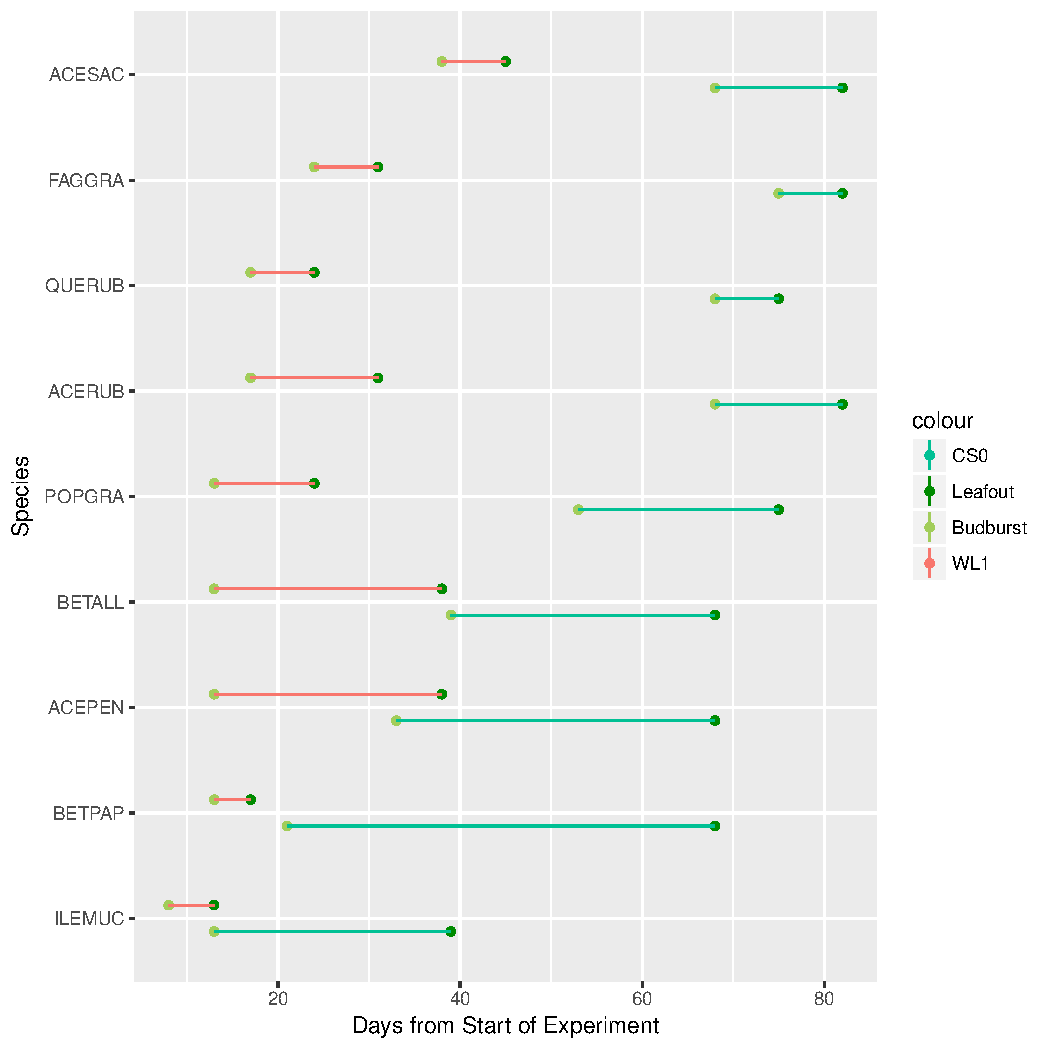
\includegraphics[width=\maxwidth]{figure/dan-1} \caption[Day of budburst and the day of leaf out for native tree species in New England]{Day of budburst and the day of leaf out for native tree species in New England. Data was collected from a growth chamber experiment using any combination of two photoperiod treatments, two forcing treatments, and three chilling treatments. The standard deviation is represented in blue for budburst and green for leaf out.}\label{fig:dan}
\end{figure}




\item According to the results, individuals that initiate budburst earlier in the season (i.e. {\textit {Betula papyrifera}} (Marsh.) and {\textit{Ilex mucronata}} (L.)) tend to begin budburst early regardless of treatment, but the treatment does affect the duration of vegetative risk significantly (Figure \ref{fig:dan}).
\item As the season progresses, treatment does not affect the duration of vegetation as much, however, the day of budburst tends to initiate later in the season with the weaker treatment effects (i.e. CS0).
\item Anova results indicate forcing temperatures and photoperiod length determine the duration of vegetative risk more than chilling requirements, which may be due to studying species within similar latitudinal range limits. 
\item Further studies are essential to investigate the interplay between chilling, forcing, and photoperiod effects on the duration of vegetative risk, especially for species occupying habitats more susceptible to false spring events. 
\end{enumerate}


\item Harvard Forest Data
\begin{enumerate}
\item Forcing temperatures in the spring affect the duration of vegetative risk: years with lower forcing temperatures and fewer growing degree days will have longer durations of vegetative risk \citep{Donnelly2017}.
\item It is therefore expected that high variation in spring temperatures (i.e. oscillating above and below the development threshold) may result in longer durations of vegetative risk.
\item Using observational data from Harvard Forest \citep{Okeefe2014}, we compared two years of data: one year that had an unusually early spring onset (2010) and another year that an unusually late spring onset (2014).
\item By comparing the durations of vegetative risk to the growing degree days for each year, we found that the number of growing degree days were highly comparable for both years, however, in 2010, the duration of vegetative risk was slightly longer overall (Figure \ref{fig:forest}). 
\item This could potentially be due to photoperiodic effects. 
\end{enumerate}
\end {enumerate}

\begin{figure} [H] 
\begin{center}
\caption{A comparison of two years of observational data investigating the effects of growing degree days on the duration of vegetative risk. The average duration of vegetative risk for 2010 was 21 +/- 3.39 days versus 17.1 +/- 1.96 days in 2014.}\label{fig:forest}
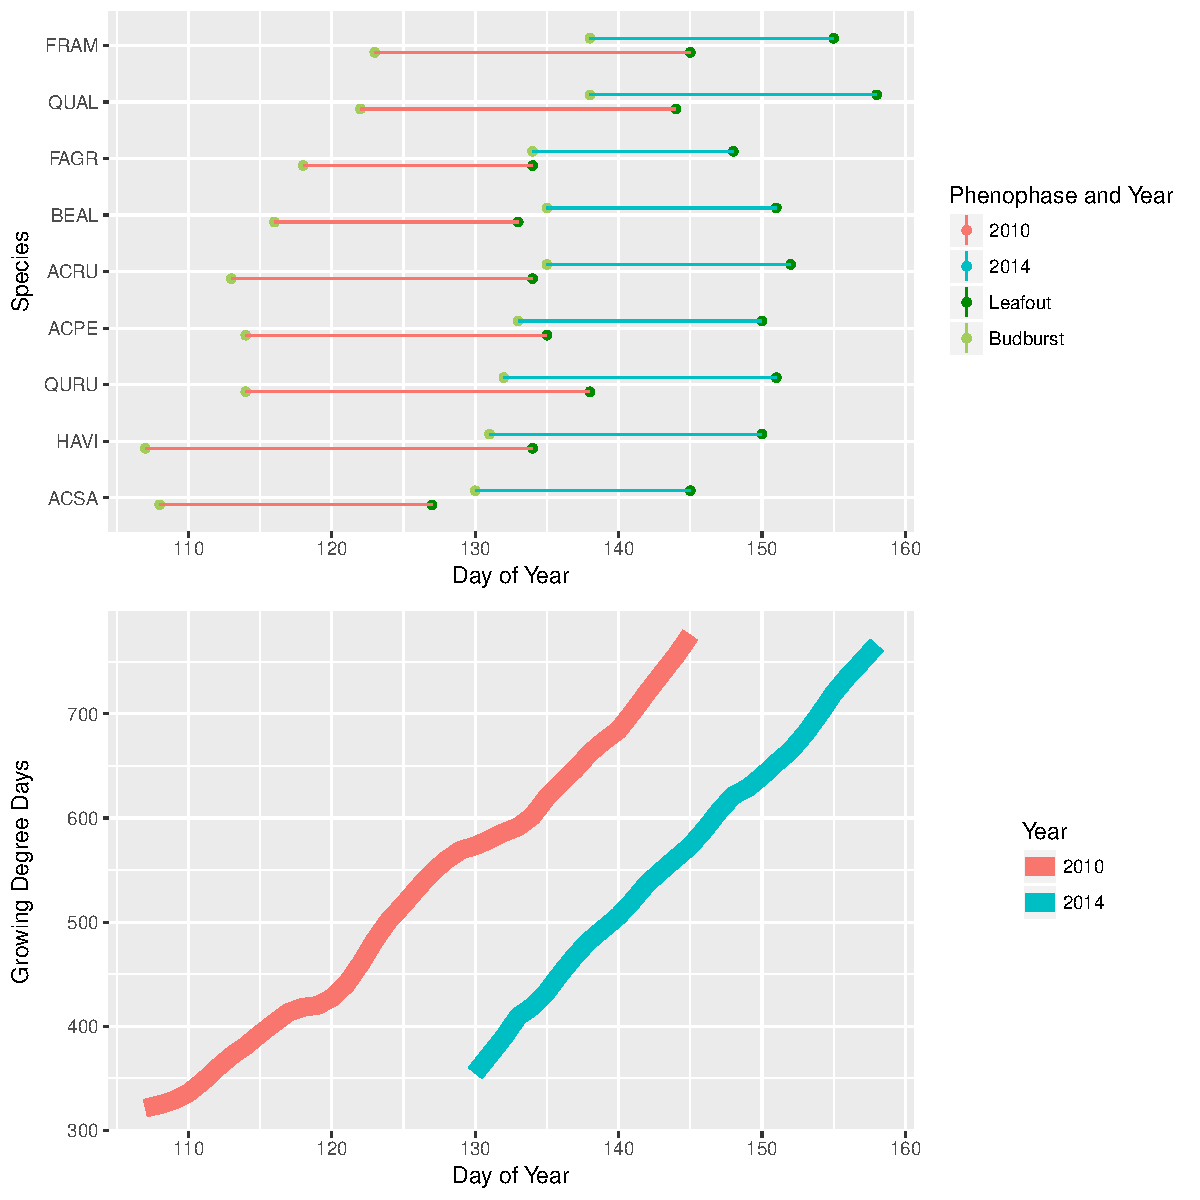
\includegraphics{..//figure/HF_gddTime.pdf}
\end{center}
\end{figure}



%%%%%%%%%%%%%%%%%%%% Regional Differences in False Spring Risk %%%%%%%%%%%%%%
\section*{Regional Differences in False Spring Risk and Temperature Thresholds}
\begin{enumerate}
\item Introduce concept of regional differences
\begin {enumerate}
\item Statement about varying durations of vegetative risk because of forest tree species demographics and climatic regimes.
\item Species distributions are largely driven by phenology \citep{Chuine2001} and photoinsensitive species are likely to outcompete photosensitive species as spring forcing temperatures continue to increase \cite{Vitasse2011,Gauzere2017}.
\item However, the climatic implications of increasing forcing temperatures could potentially lead to earlier dates of budburst and enhance the risk for frost or drought risk. 
\item These shifts in climatic regimes could vary in intensity across regions: habitats currently at risk of false spring damage could become low risk regions over time. 
\item There are discrepancies in defining a false spring event, especially with understanding damaging freezing temperatures.
\item Some regions and species may be more able to tolerate lower temperature thresholds than others (Table \ref{tab:temperature}).
\item It is crucial to gain an understanding on which climatic parameters result in false spring events, what habitats are at risk now, and what habitats will be at risk in the future. 
\item It is anticipated that most habitats will trend towards earlier spring onsets, however, the dates of last freezes will not occur at the same rate, rendering some regions to be more susceptible to false spring events in the future \citep{Labe2016}.
\item By determining the range of budburst dates for the dominant species in five archetypal climate regions, we were able to elucidate the current spatial variation of false spring risk (Figure \ref{fig:regional}).
\item We assessed the number of freezing days \citep{Schwartz1993} that occurred on average over the past 50 years within those range of dates and found that Maine has the highest risk for frost damage and Lyon, France as the lowest. 
\item Current studies focus on latitudinal and photoperiodic effects \citep{Partanen2004, Viheraaarnio2006, Caffarra2011, Gauzere2017}, however, future research should aim to integrate spatiotemporal effects more when investigating false spring risk.
\end {enumerate}
\end{enumerate}

\begin{landscape}
\begin{center}
\captionof{table}{Comparing damaging spring temperature thresholds in ecological and agronomical studies across various species and phenophases.} \label{tab:temperature} 
\footnotesize
\begin{tabular}{|c | c | c | c | c | c|}
\hline
\textbf{Sector} & \textbf{BBCH} & \textbf{Species} & \textbf{Temperature ($^{\circ}$C)} & \textbf{Type} & \textbf{Source} \\
\hline
Ecological & 9-15 & Sorbus aucuparia & -7.4 & 50\% lethality & \cite{Lenz2016} \\
\hline
Ecological & 9-15 & Prunus avium & -8.5 & 50\% lethality & \cite{Lenz2016} \\
\hline
Ecological & 9-15 & Tilia platyphyllos & -7.4 & 50\% lethality & \cite{Lenz2016} \\
\hline
Ecological & 9-15 & Acer pseudoplatanus & -6.7 & 50\% lethality & \cite{Lenz2016}\\
\hline
Ecological & 9-15 & Fagus sylvatica & -4.8 & 50\% lethality & \cite{Lenz2016}\\
\hline
Ecological & 9+ & All & -2.2 & hard & \cite{Schwartz1993}\\
\hline
Ecological & 9+ & All & -1.7 & soft & \cite{Augspurger2013} \\
\hline
Ecological & All & All & 2 SD below winter TAVG & cold-air outbreaks & \cite{Vavrus2006} \\
\hline
Ecological & 9+ & Eucalyptus pauciflora & -5.8 & elevated CO2 and temperature threshold & \cite{Barker2005} \\
\hline
Ecological & 9+ & All & -2.2 & 7 day threshold & \cite{Peterson2014} \\
\hline
Agrinomical & 9+ & All & 2 & Risk threshold for clear nights & \cite{Cannell1986} \\
\hline
Agrinomical & Floral & Vaccinium spp. & -4.4 to 0 & sprinkler protection threshold & \cite{Longstroth2012} \\
\hline
Agrinomical & 9 & Rosaceae & -7.2 & 10\% lethality & \cite{Longstroth2013}\\
\hline
Agrinomical & 9 & Rosaceae & -13.3 & 90\% lethality & \cite{Longstroth2013} \\
\hline
Agrinomical & All & All & Varies & Radiation Frost & \cite{Barlow2015} \\
\hline
Agrinomical & Floral & Wheat & -4 to -5 & 10-90\% lethality & \cite{Barlow2015} \\
\hline
Agrinomical & Vegetative & Wheat & -7 for 2hrs & 100\% lethality & \cite{Barlow2015} \\
\hline
Agrinomical & Vegetative & Rice & 4.7 & lethal limit & \cite{Sanchez2013} \\
\hline
Agrinomical & Vegetative & Corn & -1.8 & lethal limit & \cite{Sanchez2013}\\
\hline
Agrinomical & Vegetative & Wheat & -17.2 & lethal limit & \cite{Sanchez2013} \\
\hline
\end{tabular}
\end{center}
\end{landscape}
\restoregeometry


\begin{figure} [H] 
\begin{center}
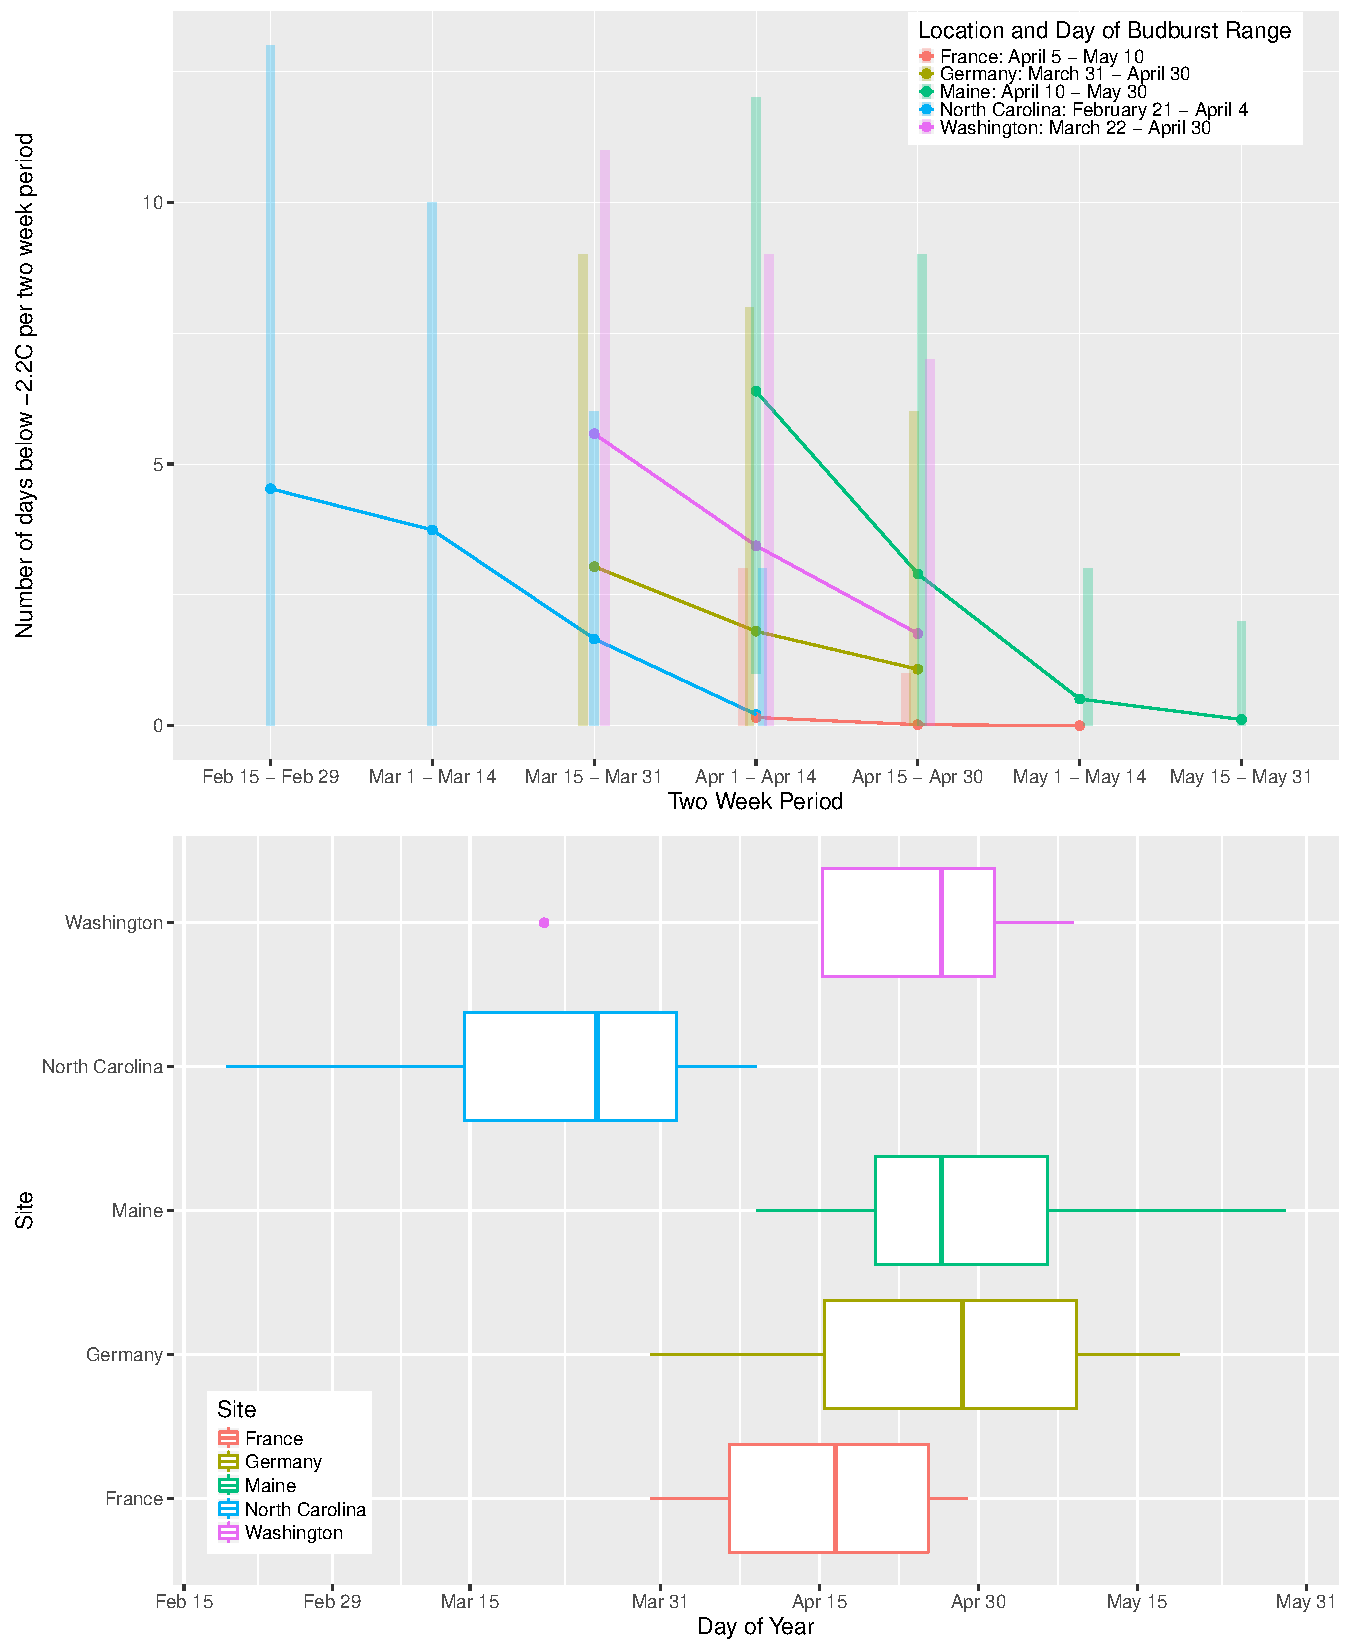
\includegraphics{..//figure/RegionalRisk.pdf}
\caption{A comparison of false spring risk across five climate regions. The data was subsetted for each region based on earliest historical spring onset date to the latest historical leafout date and was divided into biweekly time periods \citep{Schaber2005, White2009, Soudani2012, USA-NPN2016}.}\label{fig:regional} 
\end{center}
\end{figure}


%%%%%%%%%%%%%%%%%%%%% DISCUSSION AND CONCLUSION %%%%%%%%%%%%%%%%%%%%%%%%%%%%%%%%%%%%%%%%%%%
\section*{Conclusion}
\begin{enumerate}
\item Phenology is closely linked to climatic regimes \citep{Wolkovich2011} and is therefore a key indicator for the phenotypic variation for cold adpated traits and false spring risk avoidance.
\item Understanding the variation of spring onset across regions and within habitats as well as the rate of budburst will permit greater insight into false spring risk.
\item Tree species with smaller and more fragemented distribution ranges are more prone to genetic drift due to geographic barriers and higher susceptibility to stochastic events (i.e. frost and drought) \citep{Alberto2013} so gathering data on species at risk is essential. 
\item Climate change could increase the level of damage from spring frost events, especially in certain regions or for particular species, due to earlier spring onset and greater fluctuations in temperature \citep{Martin2010}. 
\item Therefore, it is essential that temperate forest tree species maintain continuous ranges in order to successfully track the changes in climate and to utilize photoperiodic and temperature cues simultaneously rather than rely strickly on photoperiodism especially along range edges \citep{Zohner2016, Gauzere2017}.
\item Future studies are necessary to investigate the relationship between phenological plasticity, the level of damage sustained from false spring events, and the duration of vegetative risk. 
\end{enumerate}




\bibliography{..//refs/SpringFreeze.bib}


\section*{Supplemental Information}
% latex table generated in R 3.3.1 by xtable 1.8-2 package
% Mon Jun 12 12:11:43 2017
\begin{table}[ht]
\centering
\begin{tabular}{rrrrr}
  \hline
  ACEPEN & Sum.Sq & Df & F value & Pr(>F) \\
 \hline
chilling & 149.41 &   2 & 1.20 & 0.30 \\ 
  forcing & 4909.59 &   1 & 78.94 & 0.00 \\ 
  photoperiod & 1309.59 &   1 & 21.06 & 0.00 \\ 
  Residuals & 6654.56 & 107 &  &  \\ 
   \hline
\end{tabular}
\end{table}
% latex table generated in R 3.3.1 by xtable 1.8-2 package
% Mon Jun 12 12:11:43 2017
\begin{table}[ht]
\centering
\begin{tabular}{rrrrr}
  \hline
  ACERUB & Sum.Sq & Df & F value & Pr(>F) \\
 \hline
chilling & 0.62 &   2 & 0.00 & 1.00 \\ 
  forcing & 1731.00 &   1 & 25.92 & 0.00 \\ 
  photoperiod & 462.78 &   1 & 6.93 & 0.01 \\ 
  Residuals & 6611.17 &  99 &  &  \\ 
   \hline
\end{tabular}
\end{table}
% latex table generated in R 3.3.1 by xtable 1.8-2 package
% Mon Jun 12 12:11:43 2017
\begin{table}[ht]
\centering
\begin{tabular}{rrrrr}
  \hline
  ACESAC & Sum.Sq & Df & F value & Pr(>F) \\
 \hline
chilling & 65.41 &   2 & 0.46 & 0.64 \\ 
  forcing & 259.14 &   1 & 3.61 & 0.06 \\ 
  photoperiod & 231.41 &   1 & 3.22 & 0.08 \\ 
  Residuals & 4524.88 &  63 &  &  \\ 
   \hline
\end{tabular}
\end{table}
% latex table generated in R 3.3.1 by xtable 1.8-2 package
% Mon Jun 12 12:11:43 2017
\begin{table}[ht]
\centering
\begin{tabular}{rrrrr}
  \hline
  BETALL & Sum.Sq & Df & F value & Pr(>F) \\
 \hline
chilling & 525.95 &   2 & 5.00 & 0.01 \\ 
  forcing & 1463.30 &   1 & 27.81 & 0.00 \\ 
  photoperiod & 632.83 &   1 & 12.03 & 0.00 \\ 
  Residuals & 6944.50 & 132 &  &  \\ 
   \hline
\end{tabular}
\end{table}
% latex table generated in R 3.3.1 by xtable 1.8-2 package
% Mon Jun 12 12:11:43 2017
\begin{table}[ht]
\centering
\begin{tabular}{rrrrr}
  \hline
  BETPAP & Sum.Sq & Df & F value & Pr(>F) \\
 \hline
chilling & 6.00 &   2 & 0.04 & 0.96 \\ 
  forcing & 1776.23 &   1 & 21.47 & 0.00 \\ 
  photoperiod & 1105.08 &   1 & 13.35 & 0.00 \\ 
  Residuals & 10509.00 & 127 &  &  \\ 
   \hline
\end{tabular}
\end{table}
% latex table generated in R 3.3.1 by xtable 1.8-2 package
% Mon Jun 12 12:11:43 2017
\begin{table}[ht]
\centering
\begin{tabular}{rrrrr}
  \hline
  FAGGRA & Sum.Sq & Df & F value & Pr(>F) \\
 \hline
chilling & 144.41 &   2 & 1.66 & 0.20 \\ 
  forcing & 611.20 &   1 & 14.04 & 0.00 \\ 
  photoperiod & 1.05 &   1 & 0.02 & 0.88 \\ 
  Residuals & 2829.78 &  65 &  &  \\ 
   \hline
\end{tabular}
\end{table}
% latex table generated in R 3.3.1 by xtable 1.8-2 package
% Mon Jun 12 12:11:43 2017
\begin{table}[ht]
\centering
\begin{tabular}{rrrrr}
  \hline
  ILEMUC & Sum.Sq & Df & F value & Pr(>F) \\
 \hline
chilling & 26.49 &   2 & 0.54 & 0.59 \\ 
  forcing & 2262.34 &   1 & 91.61 & 0.00 \\ 
  photoperiod & 1035.85 &   1 & 41.94 & 0.00 \\ 
  Residuals & 3334.05 & 135 &  &  \\ 
   \hline
\end{tabular}
\end{table}
% latex table generated in R 3.3.1 by xtable 1.8-2 package
% Mon Jun 12 12:11:43 2017
\begin{table}[ht]
\centering
\begin{tabular}{rrrrr}
  \hline
  POPGRA & Sum.Sq & Df & F value & Pr(>F) \\
 \hline
chilling & 54.63 &   2 & 0.39 & 0.68 \\ 
  forcing & 2405.73 &   1 & 34.52 & 0.00 \\ 
  photoperiod & 1019.78 &   1 & 14.63 & 0.00 \\ 
  Residuals & 6760.98 &  97 &  &  \\ 
   \hline
\end{tabular}
\end{table}
% latex table generated in R 3.3.1 by xtable 1.8-2 package
% Mon Jun 12 12:11:43 2017
\begin{table}[ht]
\centering
\begin{tabular}{rrrrr}
  \hline
  QUERUB & Sum.Sq & Df & F value & Pr(>F) \\
 \hline
chilling & 35.61 &   2 & 0.45 & 0.64 \\ 
  forcing & 680.83 &   1 & 17.34 & 0.00 \\ 
  photoperiod & 369.53 &   1 & 9.41 & 0.00 \\ 
  Residuals & 4946.29 & 126 &  &  \\ 
   \hline
\end{tabular}
\end{table}


% latex table generated in R 3.3.1 by xtable 1.8-2 package
% Mon Jun 12 12:11:44 2017
\begin{table}[ht]
\centering
\begin{tabular}{rrrrr}
  \hline
  ACEPEN & Sum.Sq & Df & F value & Pr(>F) \\
 \hline
chilling & 104.66 &   2 & 0.87 & 0.42 \\ 
  forcing & 4745.38 &   1 & 79.18 & 0.00 \\ 
  photoperiod & 1306.03 &   1 & 21.79 & 0.00 \\ 
  chilling:forcing & 63.31 &   2 & 0.53 & 0.59 \\ 
  chilling:photoperiod & 181.96 &   2 & 1.52 & 0.22 \\ 
  forcing:photoperiod & 257.63 &   1 & 4.30 & 0.04 \\ 
  Residuals & 6113.18 & 102 &  &  \\ 
   \hline
\end{tabular}
\end{table}
% latex table generated in R 3.3.1 by xtable 1.8-2 package
% Mon Jun 12 12:11:44 2017
\begin{table}[ht]
\centering
\begin{tabular}{rrrrr}
  \hline
  ACERUB & Sum.Sq & Df & F value & Pr(>F) \\
 \hline
chilling & 1.53 &   2 & 0.01 & 0.99 \\ 
  forcing & 1721.25 &   1 & 26.13 & 0.00 \\ 
  photoperiod & 381.81 &   1 & 5.80 & 0.02 \\ 
  chilling:forcing & 358.58 &   2 & 2.72 & 0.07 \\ 
  chilling:photoperiod & 37.69 &   2 & 0.29 & 0.75 \\ 
  forcing:photoperiod & 17.35 &   1 & 0.26 & 0.61 \\ 
  Residuals & 6191.98 &  94 &  &  \\ 
   \hline
\end{tabular}
\end{table}
% latex table generated in R 3.3.1 by xtable 1.8-2 package
% Mon Jun 12 12:11:44 2017
\begin{table}[ht]
\centering
\begin{tabular}{rrrrr}
  \hline
  ACESAC & Sum.Sq & Df & F value & Pr(>F) \\
 \hline
chilling & 65.78 &   2 & 0.45 & 0.64 \\ 
  forcing & 204.31 &   1 & 2.83 & 0.10 \\ 
  photoperiod & 267.24 &   1 & 3.70 & 0.06 \\ 
  chilling:forcing & 76.27 &   2 & 0.53 & 0.59 \\ 
  chilling:photoperiod & 164.28 &   2 & 1.14 & 0.33 \\ 
  forcing:photoperiod & 0.05 &   1 & 0.00 & 0.98 \\ 
  Residuals & 4194.28 &  58 &  &  \\ 
   \hline
\end{tabular}
\end{table}
% latex table generated in R 3.3.1 by xtable 1.8-2 package
% Mon Jun 12 12:11:44 2017
\begin{table}[ht]
\centering
\begin{tabular}{rrrrr}
  \hline
  BETALL & Sum.Sq & Df & F value & Pr(>F) \\
 \hline
chilling & 526.41 &   2 & 5.57 & 0.00 \\ 
  forcing & 1463.33 &   1 & 30.95 & 0.00 \\ 
  photoperiod & 632.83 &   1 & 13.38 & 0.00 \\ 
  chilling:forcing & 66.32 &   2 & 0.70 & 0.50 \\ 
  chilling:photoperiod & 226.18 &   2 & 2.39 & 0.10 \\ 
  forcing:photoperiod & 612.56 &   1 & 12.95 & 0.00 \\ 
  Residuals & 6005.50 & 127 &  &  \\ 
   \hline
\end{tabular}
\end{table}
% latex table generated in R 3.3.1 by xtable 1.8-2 package
% Mon Jun 12 12:11:44 2017
\begin{table}[ht]
\centering
\begin{tabular}{rrrrr}
  \hline
  BETPAP & Sum.Sq & Df & F value & Pr(>F) \\
 \hline
chilling & 6.07 &   2 & 0.04 & 0.96 \\ 
  forcing & 1765.57 &   1 & 21.22 & 0.00 \\ 
  photoperiod & 1101.18 &   1 & 13.24 & 0.00 \\ 
  chilling:forcing & 71.38 &   2 & 0.43 & 0.65 \\ 
  chilling:photoperiod & 62.92 &   2 & 0.38 & 0.69 \\ 
  forcing:photoperiod & 233.62 &   1 & 2.81 & 0.10 \\ 
  Residuals & 10148.80 & 122 &  &  \\ 
   \hline
\end{tabular}
\end{table}
% latex table generated in R 3.3.1 by xtable 1.8-2 package
% Mon Jun 12 12:11:44 2017
\begin{table}[ht]
\centering
\begin{tabular}{rrrrr}
  \hline
  FAGGRA & Sum.Sq & Df & F value & Pr(>F) \\
 \hline
chilling & 145.37 &   2 & 1.64 & 0.20 \\ 
  forcing & 595.26 &   1 & 13.40 & 0.00 \\ 
  photoperiod & 0.42 &   1 & 0.01 & 0.92 \\ 
  chilling:forcing & 39.45 &   2 & 0.44 & 0.64 \\ 
  chilling:photoperiod & 83.56 &   2 & 0.94 & 0.40 \\ 
  forcing:photoperiod & 35.33 &   1 & 0.80 & 0.38 \\ 
  Residuals & 2665.38 &  60 &  &  \\ 
   \hline
\end{tabular}
\end{table}
% latex table generated in R 3.3.1 by xtable 1.8-2 package
% Mon Jun 12 12:11:44 2017
\begin{table}[ht]
\centering
\begin{tabular}{rrrrr}
  \hline
  ILEMUC & Sum.Sq & Df & F value & Pr(>F) \\
 \hline
chilling & 28.03 &   2 & 0.60 & 0.55 \\ 
  forcing & 2277.73 &   1 & 97.37 & 0.00 \\ 
  photoperiod & 1033.49 &   1 & 44.18 & 0.00 \\ 
  chilling:forcing & 16.09 &   2 & 0.34 & 0.71 \\ 
  chilling:photoperiod & 106.28 &   2 & 2.27 & 0.11 \\ 
  forcing:photoperiod & 171.89 &   1 & 7.35 & 0.01 \\ 
  Residuals & 3041.00 & 130 &  &  \\ 
   \hline
\end{tabular}
\end{table}
% latex table generated in R 3.3.1 by xtable 1.8-2 package
% Mon Jun 12 12:11:44 2017
\begin{table}[ht]
\centering
\begin{tabular}{rrrrr}
  \hline
  POPGRA & Sum.Sq & Df & F value & Pr(>F) \\
 \hline
chilling & 50.56 &   2 & 0.37 & 0.69 \\ 
  forcing & 2390.66 &   1 & 35.16 & 0.00 \\ 
  photoperiod & 1016.39 &   1 & 14.95 & 0.00 \\ 
  chilling:forcing & 45.72 &   2 & 0.34 & 0.72 \\ 
  chilling:photoperiod & 152.02 &   2 & 1.12 & 0.33 \\ 
  forcing:photoperiod & 296.37 &   1 & 4.36 & 0.04 \\ 
  Residuals & 6254.69 &  92 &  &  \\ 
   \hline
\end{tabular}
\end{table}
% latex table generated in R 3.3.1 by xtable 1.8-2 package
% Mon Jun 12 12:11:44 2017
\begin{table}[ht]
\centering
\begin{tabular}{rrrrr}
  \hline
  QUERUB & Sum.Sq & Df & F value & Pr(>F) \\
 \hline
chilling & 35.70 &   2 & 0.46 & 0.63 \\ 
  forcing & 668.59 &   1 & 17.39 & 0.00 \\ 
  photoperiod & 364.39 &   1 & 9.48 & 0.00 \\ 
  chilling:forcing & 174.11 &   2 & 2.26 & 0.11 \\ 
  chilling:photoperiod & 110.91 &   2 & 1.44 & 0.24 \\ 
  forcing:photoperiod & 15.92 &   1 & 0.41 & 0.52 \\ 
  Residuals & 4652.62 & 121 &  &  \\ 
   \hline
\end{tabular}
\end{table}





\end{document}
